% Maybe this should move to progress section
\section{Medical Segmentation}
\subsection{Unet \& Friends}
This section we introduce several well known methods in medical segmentation. Unet \cite{ronneberger_u-net_2015} and its variations plays a dominant role in current medical segmentation tasks, and it is often used as a baseline model for performance evaluation in the literature.\\

Unet \cite{ronneberger_u-net_2015} is among one of the most widely used medical segmentation models since the day it was proposed. The original Unet consists of a contracting path followed by an expansive path that gives a "U" shaped architecture. The network architecture is shown in figure \ref{fig:unet-arch}.
Later this 2D model was extended to 3D version in \cite{ourselin_3d_2016} for for Kidney segmentation tasks so that the model learn features from information implicated between slices.\\
\begin{figure}
\centering
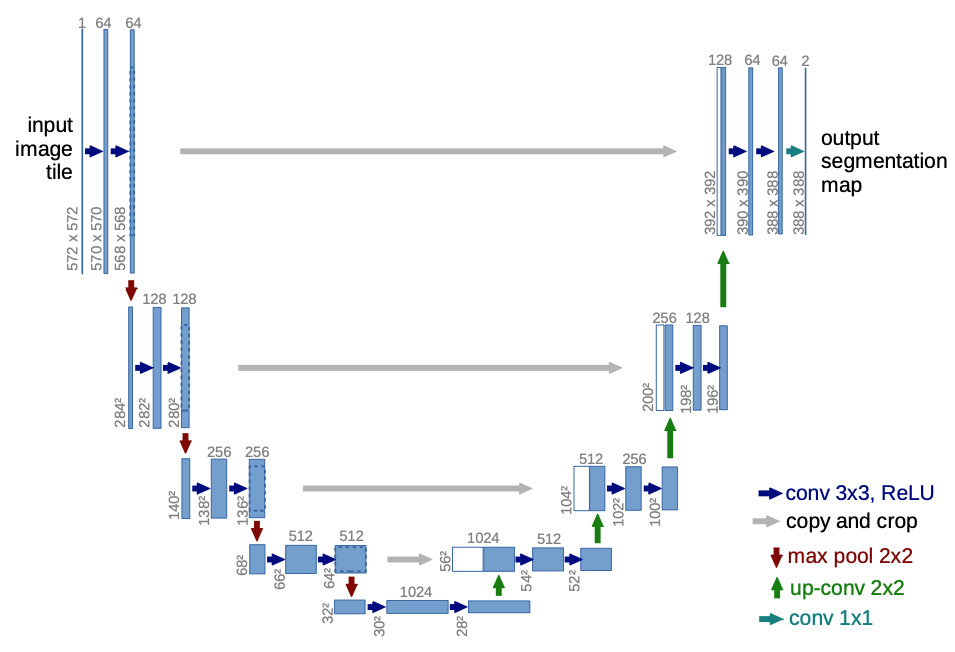
\includegraphics[width = 0.8\textwidth]{img/Unet_architecture}
\caption{Original Unet architecture in \cite{ronneberger_u-net_2015}}
\label{fig:unet-arch}
\end{figure}

VNet \cite{milletari_v-net_2016} is another 3D variation of Unet, and the network performed evaluation on prostate dataset. Each block of convolution has a residual feature that the input of the block is added to the last convolutional layer. The author argued that leverage residual structure enables network convergence in a fraction of the amount of time other network used.
%TODO insert residual structure here
\subsection{Loss functions for medical segmentation}

Loss function or objective function is a crutial component in neural network training. Segmentation tasks usually make use of \textit{Distribution loss}, \textit{Region based loss} and \textit{boundary-based} loss for training and evaluation of segmentation performance. Recent work in \cite{ma_segmentation_2020} summarized some common loss functions for segmentation. \\

\textbf{Cross entropy} (CE) measures the dissimilarity between the learned distribution and target distribution. 
$$CE = -\frac{1}{N} \sum_{i=1}^{N} \sum_{c=1}^{C} w_{c} \cdot (y_{i}^{c} \log p_{i}^{c})$$ where $y_{i}^{c}$ indicates the prediction result (correct or wrong) and $p_{i}^{c}$ denotes the predicted probability of pixel i for class c, $w_{c}$ is now 1 for original cross entropy loss.

Unet \cite{ronneberger_u-net_2015} training extend the CE by adding weight $w_{c}$. A common example for weight measurement is through the inverse proportion of observed class frequency. This modification potentially deal with imbalance class which is very common in medical domain.\\

\textbf{Dice loss} is a region based loss function that learn to optimize the Dice Coefficient (D). Vnet \cite{milletari_v-net_2016} first brought the Dice loss into machine vision community to solve the problem of highly biased prediction towards dominant area (e.g background) in medical segmentation.
 $$D=\frac{2 \sum_{i}^{N} p_{i} g_{i}}{\sum_{i}^{N} p_{i}^{2}+\sum_{i}^{N} g_{i}^{2}}$$
 Assume we segment N samples, $p_{i}$ denotes the prediction volume and $g_{i}$ denotes the ground-truth volume.
Dice loss usually require the label to be one hot encoded during training. One benefit is that Dice loss does not requires class balance methods such as weighting method in CE loss.\\

\textbf{Hausdorff Distance loss}(HD) aims to minimize the boundary distance between prediction and ground-truth segmentation masks. Similar to Dice loss, it also alleviate the class imbalance issue during training. However, paper \cite{} showed that directly minimizing Hausdorff Distance is intractable while an approximation (HD Loss) through distance transform (gray-level intensities of points inside foreground regions are changed to show the distance to the closest boundary from each point \footnote{https://homepages.inf.ed.ac.uk/rbf/HIPR2/distance.htm}).
$$L_{H D_{D T}}=\frac{1}{N} \sum_{i=1}^{N}\left[\left(s_{i}-g_{i}\right) \cdot\left(d_{G i}^{2}+d_{S i}^{2}\right)\right]$$

Paper \cite{ma_segmentation_2020} proposed that so far none of the papers in the literature provide a comprehensive comparison of the loss functions for segmentation task. Selecting loss function is still based on empirical comparison. Several works \cite{} used compound loss function that combined several loss together as training objectives overall gives good performance compared to individual loss functions.

